\begin{chapterenv}

\chapter{Three Recipes: Chatbot, Reasoner, Agent}

\section{From Techniques to Systems}

The previous chapters built a toolkit: SFT for cold-starting (Chapter 5), RLHF and PPO for preference alignment (Chapter 6), DPO and Online DPO for efficient preference learning (Chapters 7--8), reward models for feedback signals (Chapter 9), GRPO and RLOO for token-level RL (Chapter 10), verifiers and PRMs for step-level credit (Chapter 11), reasoning emergence via GRPO (Chapter 12), test-time compute for inference-time scaling (Chapter 13), self-play for self-improving systems (Chapter 14), multi-objective RL for balancing competing goals (Chapter 15), and domain-specific reward functions for code, math, and tools (Chapter 16).

The question now is: how do you assemble these ingredients into a working production system? The answer depends on what you are building. This chapter presents three recipes -- one for each major use case -- with concrete implementation guidance, expected training costs, and evaluation checklists.

\begin{figure}[!h]
\centering
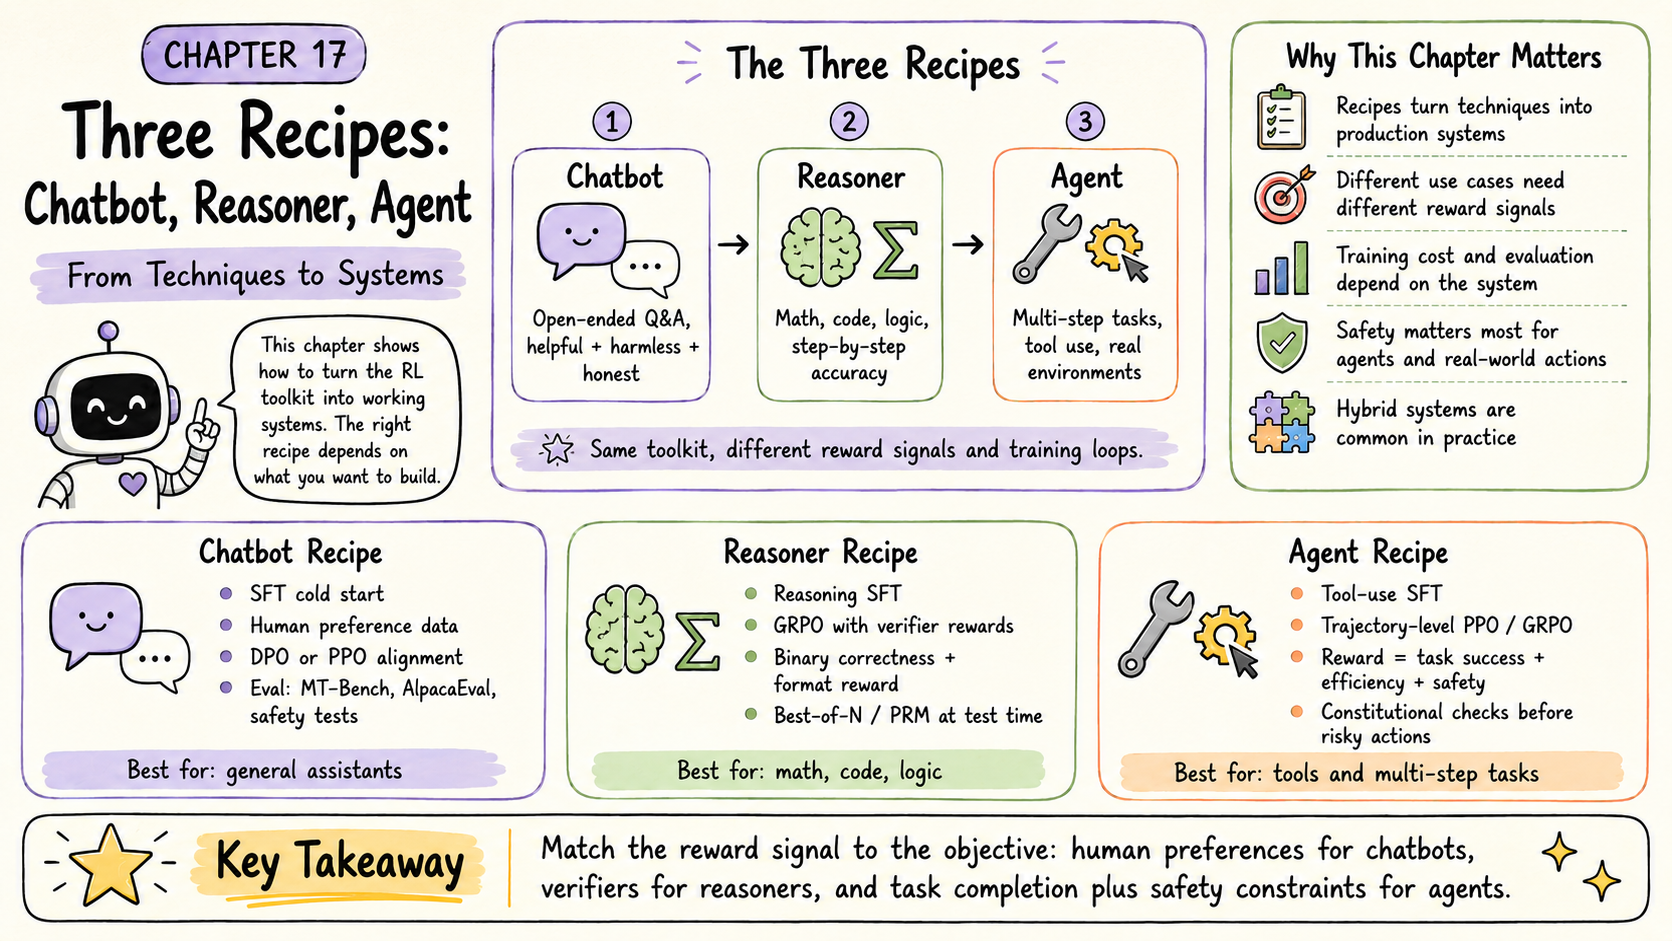
\includegraphics[width=0.88\textwidth]{images/ch17_fig01_three_recipes_intro.png}
\caption{The three production recipes at a glance -- chatbots, reasoners, and agents: same toolkit, different reward signals and training loops.}
\label{fig:ch17:three_recipes_intro}
\end{figure}

\begin{infobox}
\textbf{The three use cases.}

\textbf{Chatbot:} A conversational assistant that handles open-ended questions, follows instructions, and is safe and helpful across a wide range of topics. Success metric: user satisfaction and safety on diverse prompts.

\textbf{Reasoner:} A model that solves structured problems requiring multi-step reasoning: math, code, logic puzzles. Success metric: accuracy on held-out benchmarks (MATH, HumanEval, ARC).

\textbf{Agent:} A model that takes sequences of actions in an environment: calling tools, executing code, browsing the web, completing multi-step tasks. Success metric: task completion rate on real-world benchmarks (WebArena, AgentBench, SWE-bench).
\end{infobox}

\section{Recipe 1: The Chatbot}

A chatbot needs to be helpful, harmless, and honest across thousands of diverse prompt types. The standard RLHF pipeline (Chapters 5--6) is still the most reliable recipe for this use case.

\subsection{Phase 1 -- SFT Cold Start}

Start with a strong base model (7B--70B parameters) and fine-tune on a curated instruction-following dataset. Quality matters more than quantity here: 50,000 high-quality examples outperform 500,000 noisy ones. The SFT phase teaches the model the format and tone of a good assistant response.

\begin{tipbox}
\textbf{SFT dataset design for chatbots.}

Include diverse prompt types: factual questions, creative writing, coding help, emotional support, task completion, multi-turn dialogue. Ensure coverage of refusal cases: the model must learn \textit{when not to answer}, not just how to answer.

Data sources: ShareGPT, Alpaca, Open Assistant, or proprietary collected conversations. Filter aggressively: remove factually incorrect responses, off-tone examples, and any training data that resembles harmful content.

Target: 30,000--100,000 examples, covering 50+ distinct task types.
\end{tipbox}

\subsection{Phase 2 -- Reward Model Training}

Train a reward model (Chapter 9) on human preference comparisons. For chatbots, the reward model must capture the full HHH triad (helpful, harmless, honest) rather than a single proxy objective.

Collect preference data: present human annotators with prompt--response pairs and ask which response is better. Aim for at least 20,000 comparison pairs. Train the reward model as a binary classifier on top of a pretrained LLM using the Bradley-Terry objective (Chapter 6).

\subsection{Phase 3 -- PPO or DPO Alignment}

With the reward model in hand, align the SFT model using PPO or DPO.

\textbf{PPO (Chapter 6)} is more complex to implement and tune but generally produces stronger alignment, especially when the reward model has high variance. Key hyperparameters: KL penalty coefficient $\beta$ (start at 0.1), clip ratio $\epsilon = 0.2$, 4 rollouts per prompt.

\textbf{DPO (Chapter 7)} is simpler: convert preference pairs directly into training data and run supervised learning with the DPO loss. Faster to implement, uses less memory, and often achieves comparable performance to PPO for general chatbot use cases.

\begin{infobox}
\textbf{Chatbot recipe summary.}

\begin{tabular}{ll}
\toprule
Stage & Specification \\
\midrule
Base model & 7B--70B pretrained LLM \\
SFT data & 30k--100k instruction examples \\
Reward data & 20k--50k preference comparisons \\
RL algorithm & DPO (simpler) or PPO (stronger) \\
Evaluation & MT-Bench, AlpacaEval, safety red-teaming \\
Training cost & 8--32 A100 GPUs, 2--5 days \\
\bottomrule
\end{tabular}
\end{infobox}

\section{Recipe 2: The Reasoner}

A reasoner needs to solve structured problems correctly, not just generate plausible-sounding answers. The DeepSeek-R1 recipe (Chapter 12) is the state-of-the-art approach: use GRPO with verifiable rewards to train the model to produce correct chain-of-thought solutions.

\subsection{Phase 1 -- Reasoning SFT Cold Start}

Start with a base model that has some mathematical or code knowledge. Fine-tune on a dataset of (problem, solution) pairs where the solution includes explicit chain-of-thought reasoning. Sources: MATH, GSM8K with step-by-step solutions, APPS for code, ARC for science.

\begin{tipbox}
\textbf{Data filtering for reasoning cold start.}

Only include problems where the solution is verifiably correct. Remove solutions that skip steps or reach the right answer via incorrect reasoning (common in web-scraped data). If you cannot verify a solution's reasoning process, exclude it.

Target: 50,000--200,000 (problem, reasoning, answer) triples. Diversity of problem types within your target domain matters more than raw volume.
\end{tipbox}

\subsection{Phase 2 -- GRPO with Verifiable Rewards}

Replace the human reward model with an automated verifier (Chapter 11). For math: compare the model's final answer to the ground-truth answer using symbolic equality checking. For code: run the generated code against a test suite. For logic: evaluate formal correctness.

Apply GRPO (Chapter 10): for each problem, generate $G = 8$--$16$ response candidates, compute binary rewards (1 for correct, 0 for incorrect), normalize within the group to get advantages, and update the policy with the GRPO objective.

\begin{infobox}
\textbf{GRPO reward design for reasoning.}

\textbf{Correctness reward:} $r_{\text{correct}}(y) = 1$ if final answer matches ground truth, $0$ otherwise. This is the primary signal.

\textbf{Format reward:} $r_{\text{format}}(y) = 0.1$ if response includes a reasoning section before the final answer, $0$ otherwise. Encourages chain-of-thought without forcing a specific template.

\textbf{Length penalty:} $r_{\text{length}}(y) = -0.01 \times \max(0, |y| - L_{\max})$. Penalizes unnecessarily long responses to prevent the model from padding reasoning.

Combined: $r(y) = r_{\text{correct}}(y) + r_{\text{format}}(y) + r_{\text{length}}(y)$.
\end{infobox}

\subsection{Phase 3 -- Test-Time Scaling}

The trained reasoner is already strong. To push further, apply best-of-N with a PRM at inference time (Chapter 13). Generate $N = 8$--$64$ solutions for each problem, score each solution step-by-step with the PRM, and return the solution with the highest cumulative PRM score.

\begin{infobox}
\textbf{Reasoner recipe summary.}

\begin{tabular}{ll}
\toprule
Stage & Specification \\
\midrule
Base model & Math/code-pretrained LLM (7B--70B) \\
SFT data & 50k--200k verified (problem, CoT, answer) \\
RL algorithm & GRPO with binary verifier reward \\
Verifier & Automated (symbolic or test execution) \\
Test-time & Best-of-N with PRM scoring \\
Evaluation & MATH, AMC, HumanEval, MBPP \\
Training cost & 16--64 A100 GPUs, 3--7 days \\
\bottomrule
\end{tabular}
\end{infobox}

\section{Recipe 3: The Agent}

An agent must complete multi-step tasks in real environments: browsing the web, executing code, calling APIs, managing files. This is the hardest use case: sparse rewards, long horizons, irreversible actions, and a much larger action space than text generation.

\subsection{Phase 1 -- Tool-Use SFT}

Fine-tune on demonstrations of correct tool use: which tool to call, with what arguments, and how to interpret the result. Sources: ToolBench, AgentInstruct, or task-specific demonstrations. The SFT phase teaches the model the tool-use format before any RL.

\begin{tipbox}
\textbf{Tool-use SFT data structure.}

Each training example should follow the format: \texttt{[SYSTEM: available tools] [USER: task] [ASSISTANT: reasoning + tool call] [TOOL RESULT: output] [ASSISTANT: reasoning + tool call] ... [ASSISTANT: final answer]}. The model must learn to alternate between reasoning and action, not just generate responses.

Include examples of tool call \textit{failures} (wrong arguments, API errors) and correct recovery. An agent that has never seen a failed tool call will not know how to handle one in production.
\end{tipbox}

\subsection{Phase 2 -- Reward Shaping and RL}

Define a reward function that covers both task completion and quality of the trajectory:

$$r_{\text{agent}}(\tau) = r_{\text{task}}(s_T) + \sum_{t=1}^{T} [r_{\text{efficiency}}(a_t) + r_{\text{safety}}(a_t)]$$

where $r_{\text{task}}$ is binary task completion, $r_{\text{efficiency}}$ penalizes unnecessary tool calls, and $r_{\text{safety}}$ enforces constitutional constraints (no destructive actions without confirmation).

Apply PPO or GRPO at the trajectory level. Use the multi-objective aggregation strategies from Chapter 15: sum helpfulness rewards, enforce minimum safety thresholds at every step.

\begin{infobox}
\textbf{Agent recipe summary.}

\begin{tabular}{ll}
\toprule
Stage & Specification \\
\midrule
Base model & Strong instruction-following LLM \\
SFT data & 10k--50k tool-use demonstrations \\
RL algorithm & PPO or GRPO at trajectory level \\
Reward & Task completion + efficiency + safety \\
Evaluation & WebArena, SWE-bench, AgentBench \\
Training cost & 32--128 A100 GPUs, 5--14 days \\
\bottomrule
\end{tabular}
\end{infobox}

\subsection{Constitutional Safety for Agents}

For agents operating in real environments, apply Constitutional AI (Chapter 14) at every action step. Before executing any irreversible action (send email, delete file, purchase item), the agent performs a self-critique: does this action comply with the safety constitution? If not, reformulate.

This adds latency but is essential for production agents. A coding agent that deletes the wrong directory, or a browsing agent that makes an unintended purchase, can cause real harm. Constitutional checking is the last line of defense before the tool call executes.

\section{Choosing Your Recipe}

\begin{infobox}
\textbf{Which recipe fits your use case?}

\begin{tabular}{llll}
\toprule
Requirement & Chatbot & Reasoner & Agent \\
\midrule
Open-ended Q\&A & \checkmark & & \\
Math / code accuracy & & \checkmark & \checkmark \\
Multi-step tasks & & & \checkmark \\
Tool use & & & \checkmark \\
Low latency needed & \checkmark & & \\
Verifiable correctness & & \checkmark & \checkmark \\
Safety-critical & \checkmark & & \checkmark \\
\bottomrule
\end{tabular}

Hybrid systems are common in production: a chatbot backbone with reasoning capabilities for STEM queries, and tool-use capabilities for tasks that require external information. Start with the recipe that matches your primary use case, then layer capabilities as needed.
\end{infobox}

\section{Summary}

Three use cases, three recipes. The chatbot recipe uses SFT + human preference RM + PPO or DPO to produce a broadly helpful, safe, and honest assistant. The reasoner recipe uses SFT + GRPO with verifiable rewards + test-time PRM scoring to achieve high accuracy on structured problems. The agent recipe uses tool-use SFT + trajectory-level RL + constitutional safety checking to handle multi-step real-world tasks.

The key principle across all three: match the reward signal to the objective. Human preferences for chatbots. Verifiers for reasoners. Task completion plus safety constraints for agents. Chapter 18 covers what happens when these systems reach production scale: debugging training instabilities, scaling to larger models, and operating RL-trained systems reliably.


The companion notebooks for this chapter (\texttt{17\_recipe\_chatbot.ipynb}, \texttt{18\_recipe\_reasoner.ipynb}, \texttt{19\_recipe\_agent.ipynb}) are at \texttt{github.com/arunpshankar/packt-final} -- swap \texttt{github.com} for \texttt{githubtocolab.com} to open directly in Colab.

\end{chapterenv}
